\documentclass[11pt, a4paper]{article}
\usepackage{fontspec}
\setmainfont{Georgia}
\setmonofont[Scale=0.85]{Menlo}
\usepackage[top=2.5cm, bottom=2.5cm, left=2.8cm, right=2.8cm]{geometry}
\usepackage{microtype}
\usepackage{parskip}
\setlength{\parskip}{6pt}
\usepackage[dvipsnames,table]{xcolor}
\definecolor{bmlblue}{RGB}{0,72,144}
\definecolor{boxbg}{RGB}{242,246,252}
\definecolor{codefg}{RGB}{30,30,50}
\definecolor{codebg}{RGB}{248,248,252}
\definecolor{rulecolor}{RGB}{180,200,230}
\definecolor{warnyellow}{RGB}{255,248,220}
\definecolor{warnborder}{RGB}{204,153,0}
\definecolor{greenbg}{RGB}{240,252,240}
\definecolor{greenborder}{RGB}{80,160,80}
\definecolor{redbg}{RGB}{255,245,245}
\definecolor{redborder}{RGB}{180,60,60}
\definecolor{annotA}{RGB}{30,100,200}
\definecolor{annotB}{RGB}{180,40,40}
\definecolor{annotC}{RGB}{40,140,60}
\definecolor{annotD}{RGB}{160,80,160}
\usepackage{amsmath, amssymb, mathtools}
\usepackage{tikz}
\usetikzlibrary{shapes.geometric,arrows.meta,positioning,fit,backgrounds,calc,decorations.pathreplacing,patterns}
\usepackage{graphicx}
\usepackage{booktabs}
\usepackage{tabularx}
\usepackage{longtable}
\usepackage{array}
\newcolumntype{L}[1]{>{\raggedright\arraybackslash}p{#1}}
\newcolumntype{C}[1]{>{\centering\arraybackslash}p{#1}}
\usepackage{listings}
\lstdefinestyle{matlab}{
  language=Matlab,
  backgroundcolor=\color{codebg},
  basicstyle=\ttfamily\small\color{codefg},
  keywordstyle=\color{bmlblue}\bfseries,
  commentstyle=\color{gray}\itshape,
  stringstyle=\color{Maroon},
  numbers=left, numberstyle=\tiny\color{gray}, numbersep=8pt,
  frame=single, framerule=0.4pt, rulecolor=\color{rulecolor},
  breaklines=true, captionpos=b, showstringspaces=false, tabsize=2
}
\usepackage[most]{tcolorbox}
\newtcolorbox{notebox}{colback=greenbg,colframe=greenborder,
  fonttitle=\bfseries,title=Note,left=4pt,right=4pt,top=3pt,bottom=3pt}
\newtcolorbox{warnbox}{colback=warnyellow,colframe=warnborder,
  fonttitle=\bfseries,title=Warning,left=4pt,right=4pt,top=3pt,bottom=3pt}
\newtcolorbox{formulabox}[1]{colback=boxbg,colframe=bmlblue!50,
  fonttitle=\bfseries\color{bmlblue},title=#1,left=4pt,right=4pt,top=3pt,bottom=3pt}
\usepackage{enumitem}
\usepackage{hyperref}
\hypersetup{colorlinks=true,linkcolor=bmlblue,urlcolor=bmlblue}
\usepackage{fancyhdr}
\pagestyle{fancy}\fancyhf{}
\fancyhead[L]{\small\color{gray}BML Annotation Tables}
\fancyhead[R]{\small\color{gray}\leftmark}
\fancyfoot[C]{\small\thepage}

% Reusable TikZ style for timeline bars
\tikzset{
  annot/.style={rectangle, minimum height=0.45cm, inner sep=0pt,
                draw=#1!70, fill=#1!20, font=\tiny},
  taxis/.style={->, thick, gray!60},
  tlabel/.style={font=\tiny, gray},
  resultbar/.style={rectangle, minimum height=0.45cm, inner sep=0pt,
                    draw=annotC!80, fill=annotC!25, font=\tiny},
  removedbar/.style={rectangle, minimum height=0.45cm, inner sep=0pt,
                     draw=gray!50, fill=gray!10, font=\tiny,
                     text=gray!60},
}

\title{\textbf{BML Annotation Tables}\\[0.5em]
  {\large Complete Reference: Interval Algebra, Manipulation,}\\
  {\large Visualization, and Worked Examples}\\[0.6em]
  {\normalsize Brain Modulation Laboratory $\cdot$ MGH / University of Pittsburgh}}
\author{}
\date{April 2026}

\begin{document}
\maketitle
\tableofcontents
\newpage

% ============================================================
\section{The Annotation Table: Core Data Structure}
\label{sec:schema}
% ============================================================

\subsection{Rationale}

Every piece of timing information in BML --- a stimulus onset, a file on disk, an artifact window, a sync interval, a spike --- is stored in a single, uniform structure: the \textbf{annotation table}. This makes every function interoperable: a function that accepts an annotation table accepts \emph{any} kind of time-stamped data.

The key insight is that everything interesting in neuroscience has a \textbf{start time} and an \textbf{end time}. Even instantaneous events (a spike, a button press) are stored with \texttt{ends = starts}, so the same code handles both.

\subsection{The four mandatory columns}

\begin{center}
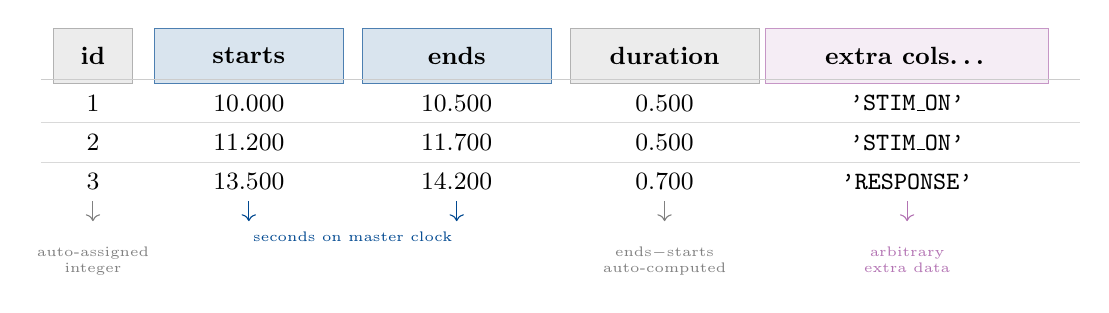
\begin{tikzpicture}[xscale=1.1]
  % Column header boxes
  \node[rectangle, draw=gray!60, fill=gray!15, minimum width=1.0cm, minimum height=0.7cm,
        font=\small\bfseries] (id) at (0,0) {id};
  \node[rectangle, draw=bmlblue!70, fill=bmlblue!15, minimum width=2.4cm, minimum height=0.7cm,
        font=\small\bfseries] (starts) at (1.8,0) {starts};
  \node[rectangle, draw=bmlblue!70, fill=bmlblue!15, minimum width=2.4cm, minimum height=0.7cm,
        font=\small\bfseries] (ends) at (4.2,0) {ends};
  \node[rectangle, draw=gray!60, fill=gray!15, minimum width=2.4cm, minimum height=0.7cm,
        font=\small\bfseries] (dur) at (6.6,0) {duration};
  \node[rectangle, draw=annotD!60, fill=annotD!10, minimum width=3.6cm, minimum height=0.7cm,
        font=\small\bfseries] (extra) at (9.4,0) {extra cols\ldots};
  % Row 1
  \node[font=\small] at (0,-0.6)   {1};
  \node[font=\small] at (1.8,-0.6)  {10.000};
  \node[font=\small] at (4.2,-0.6)  {10.500};
  \node[font=\small] at (6.6,-0.6)  {0.500};
  \node[font=\small] at (9.4,-0.6)  {\texttt{'STIM\_ON'}};
  % Row 2
  \node[font=\small] at (0,-1.1)    {2};
  \node[font=\small] at (1.8,-1.1)  {11.200};
  \node[font=\small] at (4.2,-1.1)  {11.700};
  \node[font=\small] at (6.6,-1.1)  {0.500};
  \node[font=\small] at (9.4,-1.1)  {\texttt{'STIM\_ON'}};
  % Row 3
  \node[font=\small] at (0,-1.6)    {3};
  \node[font=\small] at (1.8,-1.6)  {13.500};
  \node[font=\small] at (4.2,-1.6)  {14.200};
  \node[font=\small] at (6.6,-1.6)  {0.700};
  \node[font=\small] at (9.4,-1.6)  {\texttt{'RESPONSE'}};
  % Horizontal rules
  \draw[gray!40] (-0.6,-0.3) -- (11.4,-0.3);
  \draw[gray!30] (-0.6,-0.85) -- (11.4,-0.85);
  \draw[gray!30] (-0.6,-1.35) -- (11.4,-1.35);
  % Annotations below
  \draw[<-,gray,thin] (0,-2.1) -- (0,-1.85) node[below,font=\tiny,align=center] at (0,-2.3) {auto-assigned\\integer};
  \draw[<-,bmlblue,thin] (1.8,-2.1) -- (1.8,-1.85);
  \draw[<-,bmlblue,thin] (4.2,-2.1) -- (4.2,-1.85);
  \node[font=\tiny,bmlblue,align=center] at (3.0,-2.3) {seconds on master clock};
  \draw[<-,gray,thin] (6.6,-2.1) -- (6.6,-1.85) node[below,font=\tiny,align=center] at (6.6,-2.3) {ends$-$starts\\auto-computed};
  \draw[<-,annotD!80,thin] (9.4,-2.1) -- (9.4,-1.85) node[below,font=\tiny,align=center] at (9.4,-2.3) {arbitrary\\extra data};
\end{tikzpicture}
\end{center}

\begin{itemize}[noitemsep]
  \item \textbf{id}: unique integer per row. Auto-assigned in ascending order sorted by \texttt{starts}. Not stable across calls to \texttt{bml\_annot\_table} --- never use \texttt{id} as a persistent key.
  \item \textbf{starts}: interval start time, in seconds on the master clock.
  \item \textbf{ends}: interval end time ($\geq$ \texttt{starts}). Instantaneous events: \texttt{ends = starts}.
  \item \textbf{duration}: \texttt{ends $-$ starts}, always recomputed; never trust an existing \texttt{duration} column if \texttt{starts}/\texttt{ends} were modified.
\end{itemize}

\subsection{Creating annotation tables}

\begin{lstlisting}[style=matlab, caption={Three ways to call bml\_annot\_table}]
% 1. From a table with starts and ends columns
T = table([1.0; 2.5; 4.0], [1.5; 3.0; 4.8], ...
          'VariableNames', {'starts','ends'});
T.type = {'STIM_ON'; 'STIM_ON'; 'RESPONSE'};
annot = bml_annot_table(T);
% -> id=[1;2;3], duration=[0.5;0.5;0.8] auto-computed

% 2. From a two-column numeric matrix [starts, ends]
annot = bml_annot_table([10 10.5; 11.2 11.7; 13.5 14.2]);

% 3. From a struct
s.starts = [10; 11.2; 13.5];
s.ends   = [10.5; 11.7; 14.2];
s.type   = {'A';'A';'B'};
annot = bml_annot_table(struct2table(s));
\end{lstlisting}

\begin{warnbox}
  \texttt{bml\_annot\_table()} sorts rows by \texttt{starts} and re-numbers \texttt{id} from 1. If you add a row manually and call it again, all ids change. Use \texttt{id} only as a within-table reference, never as a cross-table key.
\end{warnbox}

% ============================================================
\section{The ROI Table and the (s1, t1, s2, t2) Coordinate System}
\label{sec:roi}
% ============================================================

\subsection{What is an ROI table?}

A \textbf{Region of Interest (ROI) table} is an annotation table extended with file metadata and \emph{sync coordinates}. Each row describes a time window within a specific file on disk.

\begin{center}
\small
\begin{tabular}{llll}
\toprule
\textbf{Column} & \textbf{Type} & \textbf{Source} & \textbf{Meaning} \\
\midrule
id, starts, ends, duration & double & annotation & Time window (master clock) \\
folder & string & filesystem & Directory containing the file \\
name & string & filesystem & Filename \\
nSamples & int & file header & Total number of samples \\
Fs & double & file header & Nominal sampling rate (Hz) \\
filetype & string & config & e.g.\ \texttt{'trellis'}, \texttt{'zoom'}, \texttt{'neuroomega'} \\
chantype & string & config & e.g.\ \texttt{'analog'}, \texttt{'digital'}, \texttt{'lfp'} \\
\midrule
\textbf{s1} & int & sync & First anchor: sample index \\
\textbf{t1} & double & sync & First anchor: master-clock time of sample s1 \\
\textbf{s2} & int & sync & Second anchor: sample index \\
\textbf{t2} & double & sync & Second anchor: master-clock time of sample s2 \\
\bottomrule
\end{tabular}
\end{center}

\subsection{The linear coordinate map}

The four sync coordinates \texttt{(s1, t1, s2, t2)} define an affine map between sample index space and master-clock time:

\begin{formulabox}{Index-to-time conversion}
\[
F_{s,\mathrm{eff}} = \frac{s_2 - s_1}{t_2 - t_1}, \qquad
t(i) = \frac{i - s_1}{F_{s,\mathrm{eff}}} + t_1 - \frac{0.5}{F_{s,\mathrm{eff}}}
     = \frac{i}{F_{s,\mathrm{eff}}} - \frac{0.5}{F_{s,\mathrm{eff}}} + \frac{s_2 t_1 - t_2 s_1}{s_2 - s_1}
\]
\end{formulabox}

\begin{formulabox}{Time-to-index conversion}
\[
i(t) = \mathrm{round}\!\left(\frac{t_2 s_1 - s_2 t_1 + (s_2 - s_1)\,t}{t_2 - t_1}\right)
\]
\end{formulabox}

\subsection{Why sample midpoints?}

Sample $i$ occupies the time window $\bigl[\tfrac{i-1}{F_s},\;\tfrac{i}{F_s}\bigr)$. Its \emph{midpoint} is $\tfrac{i}{F_s} - \tfrac{0.5}{F_s}$. The coordinates \texttt{t1} and \texttt{t2} refer to the midpoints of samples \texttt{s1} and \texttt{s2}, respectively.

This matters because: if you know the start of a 30 kHz file is $t_{\rm start}$, then sample 1 starts at $t_{\rm start}$ but its midpoint (what \texttt{t1} records) is $t_{\rm start} + \tfrac{0.5}{30000}$. The default initialization is:

\[
s_1 = 1,\quad t_1 = \texttt{starts} + \frac{0.5}{F_s},\quad
s_2 = N_{\rm samples},\quad t_2 = \texttt{ends} - \frac{0.5}{F_s}
\]

\begin{center}
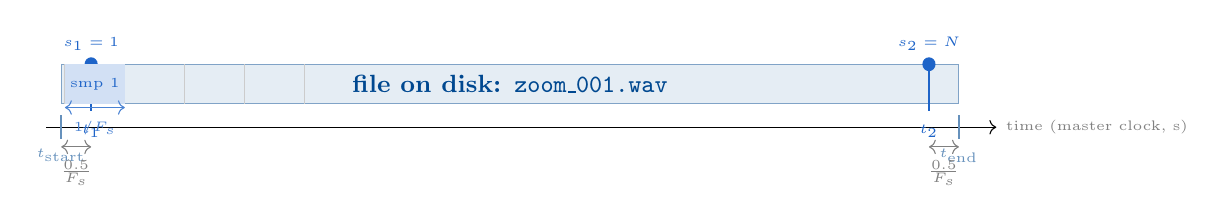
\begin{tikzpicture}[xscale=0.95]
  % File bar
  \fill[bmlblue!10] (0,0) rectangle (12,0.5);
  \draw[bmlblue!50] (0,0) rectangle (12,0.5);
  \node[font=\small\bfseries,bmlblue] at (6,0.25) {file on disk: \texttt{zoom\_001.wav}};
  % Time axis
  \draw[->] (-0.2,-0.3) -- (12.5,-0.3) node[right,font=\tiny,gray] {time (master clock, s)};
  % Tick marks at file boundaries
  \draw[thick,bmlblue!60] (0,-0.15)--(0,-0.45) node[below,font=\tiny] {$t_{\rm start}$};
  \draw[thick,bmlblue!60] (12,-0.15)--(12,-0.45) node[below,font=\tiny] {$t_{\rm end}$};
  % s1 marker
  \draw[thick,annotA] (0.4,0.5)--(0.4,-0.1);
  \fill[annotA] (0.4,0.5) circle (2.5pt);
  \node[above,font=\tiny\bfseries,annotA] at (0.4,0.55) {$s_1=1$};
  \node[below,font=\tiny,annotA] at (0.4,-0.15) {$t_1$};
  % s2 marker
  \draw[thick,annotA] (11.6,0.5)--(11.6,-0.1);
  \fill[annotA] (11.6,0.5) circle (2.5pt);
  \node[above,font=\tiny\bfseries,annotA] at (11.6,0.55) {$s_2=N$};
  \node[below,font=\tiny,annotA] at (11.6,-0.15) {$t_2$};
  % Half-sample arrows
  \draw[<->,thin,gray] (0,-0.55)--(0.4,-0.55);
  \node[below,font=\tiny,gray] at (0.2,-0.6) {$\tfrac{0.5}{F_s}$};
  \draw[<->,thin,gray] (11.6,-0.55)--(12,-0.55);
  \node[below,font=\tiny,gray] at (11.8,-0.6) {$\tfrac{0.5}{F_s}$};
  % Sample zoom inset
  \foreach \s in {0,0.8,1.6,2.4,3.2} {
    \draw[gray!40] (\s+0.05,0)--(\s+0.05,0.5);
  }
  \fill[annotA!20] (0.05,0) rectangle (0.85,0.5);
  \node[font=\tiny,annotA] at (0.45,0.25) {smp 1};
  \draw[<->,thin,annotA!80] (0.05,-0.05)--(0.85,-0.05);
  \node[below,font=\tiny,annotA!80] at (0.45,-0.1) {$1/F_s$};
\end{tikzpicture}
\end{center}

\begin{lstlisting}[style=matlab, caption={Building and using an ROI table}]
% Build from file scan
roi = bml_roi_table(bml_info_raw(struct('folder','/data/p001/s01')));

% Default coordinates:
% roi.s1 = 1 (first sample)
% roi.t1 = roi.starts + 0.5/roi.Fs   (midpoint of sample 1)
% roi.s2 = roi.nSamples
% roi.t2 = roi.ends - 0.5/roi.Fs     (midpoint of last sample)

% After synchronization, t1/t2 are updated to master-clock times.
% Convert between sample index and time:
t = bml_idx2time(roi(1,:), 15000);   % time of sample 15000
i = bml_time2idx(roi(1,:), 52312.5); % sample nearest to 52312.5 s
\end{lstlisting}

% ============================================================
\section{Creating and Loading Annotation Tables}
\label{sec:io}
% ============================================================

\subsection{From scratch}

\begin{lstlisting}[style=matlab]
% Minimal: just starts and ends
spikes = bml_annot_table(table([1.2;1.8;2.4],[1.2;1.8;2.4],...
  'VariableNames',{'starts','ends'}));

% With extra columns
trials = table([10;20;30], [10.5;20.5;30.5], {'go';'nogo';'go'}, [1;2;3],...
  'VariableNames',{'starts','ends','trial_type','value'});
trials = bml_annot_table(trials);
\end{lstlisting}

\subsection{From BIDS TSV files (\texttt{bml\_annot\_read\_tsv})}

BIDS event files use \texttt{onset} (seconds from task start) and \texttt{duration} columns. \texttt{bml\_annot\_read\_tsv} renames \texttt{onset}$\to$\texttt{starts} and computes \texttt{ends = starts + duration}.

\begin{lstlisting}[style=matlab]
events = bml_annot_read_tsv( ...
  'sub-DM1001_ses-intraop_task-speech_events.tsv');
% Columns: id, starts, ends, duration, trial_type, response_time, ...
% Also extracts sub/ses/task from filename if AppendColsFromFilename=true

% Write back after sync:
bml_annot_write_tsv(events_synced, 'sub-DM1001_...-sync.tsv');
% Renames starts->onset, drops id, writes tab-delimited
\end{lstlisting}

\subsection{From FieldTrip event structs (\texttt{bml\_event2annot})}

\begin{lstlisting}[style=matlab]
% Read Ripple (Trellis) events
ft_events = ft_read_event(fullfile(roi.folder{1},roi.name{1}));

cfg = [];
cfg.roi    = roi(strcmp(roi.filetype,'trellis'),:);
cfg.Fs     = 30000;
annot_events = bml_event2annot(cfg, ft_events);
% Columns: id, starts, ends, duration, type, value, sample
% sample = raw sample index; starts/ends = master-clock seconds via roi

% Quick shortcut used throughout BML:
master_events = bml_event2annot([], bml_read_event(trellis_roi));
\end{lstlisting}

\subsection{Scanning a folder to build the initial ROI table}

\begin{lstlisting}[style=matlab]
% Step 1: scan folder, infer file type from extension/name pattern
info = bml_info_raw(struct('folder', '/data/p001/s01', ...
                           'filetype', {'trellis','zoom','neuroomega'}));

% Step 2: create ROI table with default sync coordinates
roi = bml_roi_table(info);

% roi now has one row per file, with:
%   s1=1, t1=starts+0.5/Fs  (OS timestamps, unreliable)
%   s2=nSamples, t2=ends-0.5/Fs
% Sync functions update t1/t2 to master-clock times.
\end{lstlisting}

% ============================================================
\section{bml\_annot\_extend --- Temporal Dilation and Erosion}
\label{sec:extend}
% ============================================================

\subsection{Rationale}

Many analysis steps need a \emph{window around} an event rather than the event itself. \texttt{bml\_annot\_extend} adds (or subtracts) time on either side of every row, without touching other columns.

\begin{formulabox}{Extension rule}
$\texttt{starts}_{\rm new} = \texttt{starts} - \texttt{ext1},\qquad
 \texttt{ends}_{\rm new} = \texttt{ends} + \texttt{ext2}$

Positive = expand outward. Negative = shrink inward (erosion).
\end{formulabox}

\begin{center}
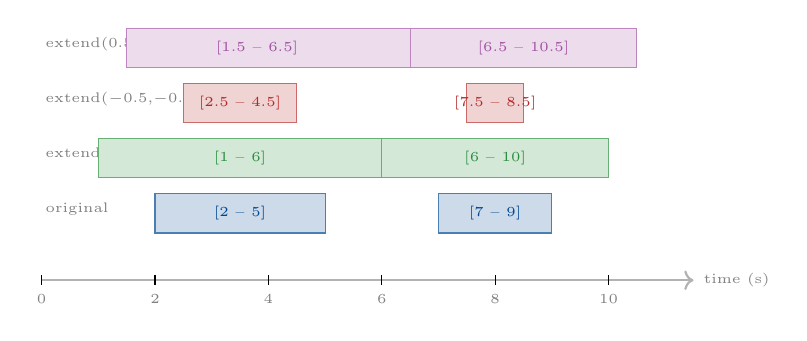
\begin{tikzpicture}[xscale=0.72]
  \draw[taxis] (0,0)--(11.5,0) node[right,font=\tiny,gray]{time (s)};
  \foreach \x in {0,2,...,10} \draw (\x,0.06)--(\x,-0.06) node[tlabel,below]{\x};
  % Original
  \node[font=\tiny,gray,right] at (-0.1,0.9) {original};
  \fill[bmlblue!20] (2,0.6) rectangle (5,1.1);
  \draw[bmlblue!70] (2,0.6) rectangle (5,1.1);
  \node[font=\tiny,bmlblue] at (3.5,0.85) {[2 -- 5]};
  \fill[bmlblue!20] (7,0.6) rectangle (9,1.1);
  \draw[bmlblue!70] (7,0.6) rectangle (9,1.1);
  \node[font=\tiny,bmlblue] at (8,0.85) {[7 -- 9]};
  % Expanded +1
  \node[font=\tiny,gray,right] at (-0.1,1.6) {extend(+1,+1)};
  \fill[annotC!20] (1,1.3) rectangle (6,1.8);
  \draw[annotC!70] (1,1.3) rectangle (6,1.8);
  \node[font=\tiny,annotC] at (3.5,1.55) {[1 -- 6]};
  \fill[annotC!20] (6,1.3) rectangle (10,1.8);
  \draw[annotC!70] (6,1.3) rectangle (10,1.8);
  \node[font=\tiny,annotC] at (8,1.55) {[6 -- 10]};
  % Contracted -0.5
  \node[font=\tiny,gray,right] at (-0.1,2.3) {extend($-$0.5,$-$0.5)};
  \fill[annotB!20] (2.5,2.0) rectangle (4.5,2.5);
  \draw[annotB!70] (2.5,2.0) rectangle (4.5,2.5);
  \node[font=\tiny,annotB] at (3.5,2.25) {[2.5 -- 4.5]};
  \fill[annotB!20] (7.5,2.0) rectangle (8.5,2.5);
  \draw[annotB!70] (7.5,2.0) rectangle (8.5,2.5);
  \node[font=\tiny,annotB] at (8,2.25) {[7.5 -- 8.5]};
  % Asymmetric
  \node[font=\tiny,gray,right] at (-0.1,3.0) {extend(0.5,1.5) asymmetric};
  \fill[annotD!20] (1.5,2.7) rectangle (6.5,3.2);
  \draw[annotD!70] (1.5,2.7) rectangle (6.5,3.2);
  \node[font=\tiny,annotD] at (3.8,2.95) {[1.5 -- 6.5]};
  \fill[annotD!20] (6.5,2.7) rectangle (10.5,3.2);
  \draw[annotD!70] (6.5,2.7) rectangle (10.5,3.2);
  \node[font=\tiny,annotD] at (8.5,2.95) {[6.5 -- 10.5]};
\end{tikzpicture}
\end{center}

\begin{lstlisting}[style=matlab]
% Add 0.5 s context on each side of every trial
trial_windows = bml_annot_extend(trials, 0.5);

% Pre-stimulus baseline: 0.5 s ending at stimulus onset
baseline = bml_annot_extend(stim_events, 0.5, 0);
% Now baseline.ends == stim_events.starts, baseline.starts == stim_events.starts - 0.5

% Shrink (erode) artifact windows by 50 ms to be conservative
artifacts_trimmed = bml_annot_extend(artifacts, -0.05);

% Asymmetric: 1 s before onset, 2 s after
analysis_win = bml_annot_extend(stim_events, 1.0, 2.0);

% Sync coarsetol: expand the ROI window to capture master events
% that might fall ±100 s outside the file OS timestamps
roi_expanded = bml_annot_extend(roi_file, 100);
\end{lstlisting}

% ============================================================
\section{bml\_annot\_filter / filterout --- Selection by Time Window}
\label{sec:filter}
% ============================================================

\subsection{Rationale}

Often you have a table of events and a table of windows, and you want to keep only the events that fall inside the windows (or remove those that overlap bad periods). This is the most common single operation in a BML pipeline.

\subsection{Overlap condition}

Two intervals $[a_1, a_2]$ and $[b_1, b_2]$ overlap if and only if:
\begin{formulabox}{Overlap condition}
$a_1 < b_2 \;\;\text{AND}\;\; a_2 > b_1$

(They overlap when neither is entirely before the other)
\end{formulabox}

With \texttt{cfg.overlap = f}: additionally require $|a \cap b| / |a| \geq f$.

\begin{center}
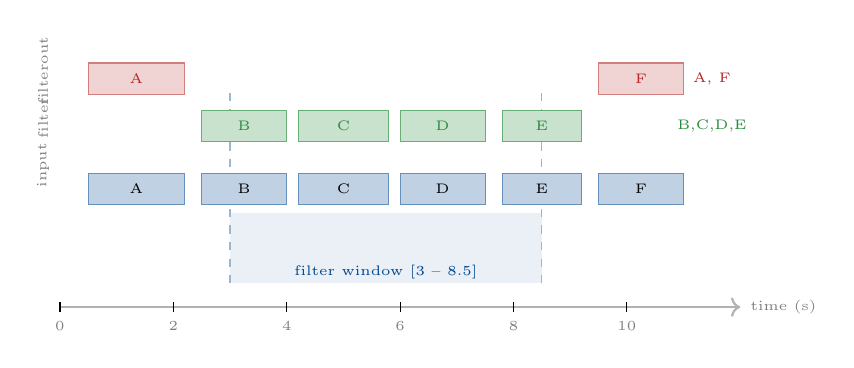
\begin{tikzpicture}[xscale=0.72]
  \draw[taxis] (0,0)--(12,0) node[right,font=\tiny,gray]{time (s)};
  \foreach \x in {0,2,...,10} \draw (\x,0.06)--(\x,-0.06) node[tlabel,below]{\x};

  % Filter region (shaded background)
  \fill[bmlblue!8] (3,0.3) rectangle (8.5,1.2);
  \draw[bmlblue!40,dashed] (3,0.3)--(3,2.8);
  \draw[bmlblue!40,dashed] (8.5,0.3)--(8.5,2.8);
  \node[font=\tiny,bmlblue] at (5.75,0.45) {filter window [3 -- 8.5]};

  % Input annotations (6 bars)
  \node[font=\tiny,gray] at (-0.3,1.8) {\rotatebox{90}{input}};
  \fill[bmlblue!25] (0.5,1.3) rectangle (2.2,1.7);  \draw[bmlblue!60] (0.5,1.3) rectangle (2.2,1.7);
  \node[font=\tiny] at (1.35,1.5) {A};
  \fill[bmlblue!25] (2.5,1.3) rectangle (4.0,1.7);  \draw[bmlblue!60] (2.5,1.3) rectangle (4.0,1.7);
  \node[font=\tiny] at (3.25,1.5) {B};  % overlaps filter
  \fill[bmlblue!25] (4.2,1.3) rectangle (5.8,1.7);  \draw[bmlblue!60] (4.2,1.3) rectangle (5.8,1.7);
  \node[font=\tiny] at (5.0,1.5) {C};   % inside filter
  \fill[bmlblue!25] (6.0,1.3) rectangle (7.5,1.7);  \draw[bmlblue!60] (6.0,1.3) rectangle (7.5,1.7);
  \node[font=\tiny] at (6.75,1.5) {D};  % inside filter
  \fill[bmlblue!25] (7.8,1.3) rectangle (9.2,1.7);  \draw[bmlblue!60] (7.8,1.3) rectangle (9.2,1.7);
  \node[font=\tiny] at (8.5,1.5) {E};   % overlaps filter
  \fill[bmlblue!25] (9.5,1.3) rectangle (11,1.7);   \draw[bmlblue!60] (9.5,1.3) rectangle (11,1.7);
  \node[font=\tiny] at (10.25,1.5) {F}; % outside filter

  % filter result
  \node[font=\tiny,gray] at (-0.3,2.4) {\rotatebox{90}{filter}};
  \fill[annotC!25] (2.5,2.1) rectangle (4.0,2.5);  \draw[annotC!70] (2.5,2.1) rectangle (4.0,2.5);
  \node[font=\tiny,annotC] at (3.25,2.3) {B};
  \fill[annotC!25] (4.2,2.1) rectangle (5.8,2.5);  \draw[annotC!70] (4.2,2.1) rectangle (5.8,2.5);
  \node[font=\tiny,annotC] at (5.0,2.3) {C};
  \fill[annotC!25] (6.0,2.1) rectangle (7.5,2.5);  \draw[annotC!70] (6.0,2.1) rectangle (7.5,2.5);
  \node[font=\tiny,annotC] at (6.75,2.3) {D};
  \fill[annotC!25] (7.8,2.1) rectangle (9.2,2.5);  \draw[annotC!70] (7.8,2.1) rectangle (9.2,2.5);
  \node[font=\tiny,annotC] at (8.5,2.3) {E};
  % filterout result
  \node[font=\tiny,gray] at (-0.3,3.0) {\rotatebox{90}{filterout}};
  \fill[annotB!20] (0.5,2.7) rectangle (2.2,3.1);  \draw[annotB!60] (0.5,2.7) rectangle (2.2,3.1);
  \node[font=\tiny,annotB] at (1.35,2.9) {A};
  \fill[annotB!20] (9.5,2.7) rectangle (11,3.1);   \draw[annotB!60] (9.5,2.7) rectangle (11,3.1);
  \node[font=\tiny,annotB] at (10.25,2.9) {F};

  % Labels
  \node[font=\tiny,annotC] at (11.5,2.3) {B,C,D,E};
  \node[font=\tiny,annotB] at (11.5,2.9) {A, F};
\end{tikzpicture}
\end{center}

\textbf{Key point}: \texttt{bml\_annot\_filter} keeps the rows of \texttt{annot} intact (start/end times are not clipped). It is a \emph{selection} operation, not a clip. Use \texttt{bml\_annot\_intersect} if you also want to clip to the filter boundary.

\begin{lstlisting}[style=matlab]
% Keep only trials within the session window
session = bml_annot_table(table(52300, 52600, 'VariableNames',{'starts','ends'}));
trials_in_session = bml_annot_filter(trials, session);

% Remove trials that overlap any artifact
clean_trials = bml_annot_filterout(trials, artifacts);

% Keep only trials where >= 50% of the trial is inside the analysis window
cfg = []; cfg.overlap = 0.5;
mostly_inside = bml_annot_filter(cfg, trials, analysis_window);

% Restrict master events to ±100s of a specific file (sync coarsetol pattern)
file_window = bml_annot_extend(roi(3,:), 100); % expand file ROI by 100s
local_events = bml_annot_filter(master_events, file_window);
\end{lstlisting}

% ============================================================
\section{bml\_annot\_intersect --- Temporal Intersection}
\label{sec:intersect}
% ============================================================

\subsection{Rationale}

\texttt{bml\_annot\_filter} selects whole rows; \texttt{bml\_annot\_intersect} \emph{clips} them to the overlap region. The result intervals are shorter than either input. Crucially, it records where each output interval came from (\texttt{x\_id}, \texttt{y\_id}).

\begin{formulabox}{Intersection of two intervals}
$[a_1,a_2] \cap [b_1,b_2] = [\max(a_1,b_1),\;\min(a_2,b_2)]$\\[3pt]
Valid (non-empty) only when $\max(a_1,b_1) < \min(a_2,b_2)$.
\end{formulabox}

\begin{center}
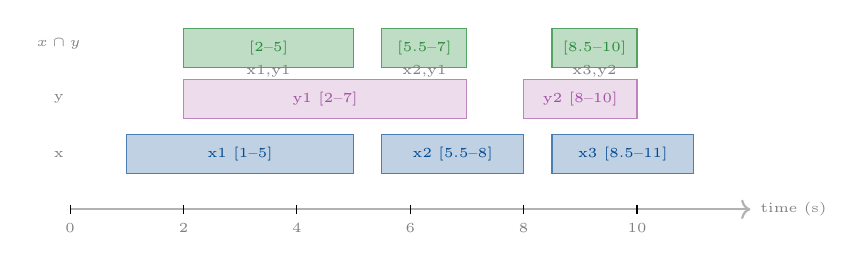
\begin{tikzpicture}[xscale=0.72]
  \draw[taxis] (0,-0.2)--(12,-0.2) node[right,font=\tiny,gray]{time (s)};
  \foreach \x in {0,2,...,10} \draw (\x,-0.14)--(\x,-0.26) node[tlabel,below]{\x};
  % x bars
  \node[font=\tiny,gray] at (-0.2,0.5) {x};
  \fill[bmlblue!25] (1,0.25) rectangle (5,0.75);   \draw[bmlblue!70] (1,0.25) rectangle (5,0.75);
  \node[font=\tiny,bmlblue] at (3,0.5) {x1 [1--5]};
  \fill[bmlblue!25] (5.5,0.25) rectangle (8,0.75); \draw[bmlblue!70] (5.5,0.25) rectangle (8,0.75);
  \node[font=\tiny,bmlblue] at (6.75,0.5) {x2 [5.5--8]};
  \fill[bmlblue!25] (8.5,0.25) rectangle (11,0.75);\draw[bmlblue!70] (8.5,0.25) rectangle (11,0.75);
  \node[font=\tiny,bmlblue] at (9.75,0.5) {x3 [8.5--11]};
  % y bars
  \node[font=\tiny,gray] at (-0.2,1.2) {y};
  \fill[annotD!20] (2,0.95) rectangle (7,1.45);    \draw[annotD!70] (2,0.95) rectangle (7,1.45);
  \node[font=\tiny,annotD] at (4.5,1.2) {y1 [2--7]};
  \fill[annotD!20] (8,0.95) rectangle (10,1.45);   \draw[annotD!70] (8,0.95) rectangle (10,1.45);
  \node[font=\tiny,annotD] at (9,1.2) {y2 [8--10]};
  % Intersection result
  \node[font=\tiny,gray] at (-0.2,1.9) {$x \cap y$};
  % x1 ∩ y1 = [2,5]
  \fill[annotC!30] (2,1.6) rectangle (5,2.1);      \draw[annotC!80] (2,1.6) rectangle (5,2.1);
  \node[font=\tiny,annotC] at (3.5,1.85) {[2--5]};
  \node[font=\tiny,gray] at (3.5,1.55) {x1,y1};
  % x2 ∩ y1 = [5.5,7]
  \fill[annotC!30] (5.5,1.6) rectangle (7,2.1);    \draw[annotC!80] (5.5,1.6) rectangle (7,2.1);
  \node[font=\tiny,annotC] at (6.25,1.85) {[5.5--7]};
  \node[font=\tiny,gray] at (6.25,1.55) {x2,y1};
  % x3 ∩ y2 = [8.5,10]
  \fill[annotC!30] (8.5,1.6) rectangle (10,2.1);   \draw[annotC!80] (8.5,1.6) rectangle (10,2.1);
  \node[font=\tiny,annotC] at (9.25,1.85) {[8.5--10]};
  \node[font=\tiny,gray] at (9.25,1.55) {x3,y2};
\end{tikzpicture}
\end{center}

\textbf{Note}: x2 overlaps y1 only partially ([5.5--7], not [5.5--8]). x1 and x3 have no intersection with y2; x3 overlaps y2 at [8.5--10], not [8.5--11].

\begin{lstlisting}[style=matlab]
% Basic intersection: clips trials to session windows
clipped = bml_annot_intersect(trials, session_windows);
% clipped has x_id (trial id) and y_id (session id) columns

% Keep columns from both tables (cfg.keep = 'both', default)
cfg = []; cfg.keep = 'both';
overlap_info = bml_annot_intersect(cfg, trials, artifacts);
% overlap_info.trials_id, overlap_info.artifacts_id, plus all extra columns

% Keep only x columns (strip y metadata from output)
cfg = []; cfg.keep = 'x';
clipped_trials = bml_annot_intersect(cfg, trials, session_windows);

% Per-channel intersection (each channel has its own artifact list)
cfg = []; cfg.groupby = 'channel';
per_ch = bml_annot_intersect(cfg, spikes, artifacts_per_channel);
\end{lstlisting}

% ============================================================
\section{bml\_annot\_union --- Temporal Union}
\label{sec:union}
% ============================================================

\subsection{Rationale}

Merge overlapping or touching intervals into the fewest possible non-overlapping intervals. Used to combine artifact lists from multiple sources, merge session windows, etc.

\begin{formulabox}{Merging condition}
Intervals $[a_1,a_2]$ and $[b_1,b_2]$ (with $b_1 \geq a_1$) are merged when:\\[3pt]
$b_1 \leq a_2 + \texttt{timetol}$\quad(they touch or overlap within tolerance)
\end{formulabox}

\begin{center}
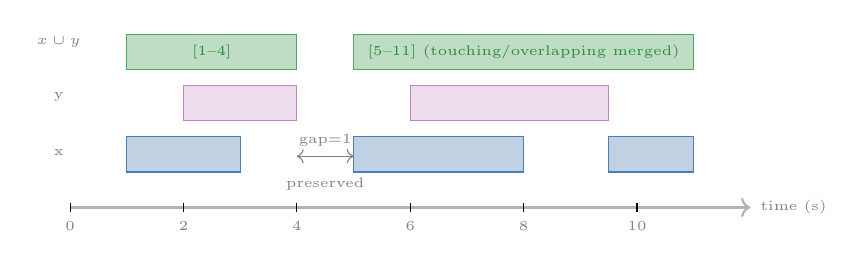
\begin{tikzpicture}[xscale=0.72]
  \draw[taxis] (0,-0.2)--(12,-0.2) node[right,font=\tiny,gray]{time (s)};
  \foreach \x in {0,2,...,10} \draw (\x,-0.14)--(\x,-0.26) node[tlabel,below]{\x};
  % x bars
  \node[font=\tiny,gray] at (-0.2,0.5) {x};
  \fill[bmlblue!25] (1,0.25) rectangle (3,0.7);   \draw[bmlblue!70] (1,0.25) rectangle (3,0.7);
  \fill[bmlblue!25] (5,0.25) rectangle (8,0.7);   \draw[bmlblue!70] (5,0.25) rectangle (8,0.7);
  \fill[bmlblue!25] (9.5,0.25) rectangle (11,0.7);\draw[bmlblue!70] (9.5,0.25) rectangle (11,0.7);
  % y bars
  \node[font=\tiny,gray] at (-0.2,1.2) {y};
  \fill[annotD!20] (2,0.9) rectangle (4,1.35);     \draw[annotD!70] (2,0.9) rectangle (4,1.35);
  \fill[annotD!20] (6,0.9) rectangle (9.5,1.35);   \draw[annotD!70] (6,0.9) rectangle (9.5,1.35);
  % Union result
  \node[font=\tiny,gray] at (-0.2,1.9) {$x \cup y$};
  \fill[annotC!30] (1,1.55) rectangle (4,2.0);     \draw[annotC!80] (1,1.55) rectangle (4,2.0);
  \node[font=\tiny,annotC] at (2.5,1.775) {[1--4]};
  \fill[annotC!30] (5,1.55) rectangle (11,2.0);    \draw[annotC!80] (5,1.55) rectangle (11,2.0);
  \node[font=\tiny,annotC] at (8,1.775) {[5--11]  (touching/overlapping merged)};
  % Gap annotation
  \draw[<->,thin,gray] (4,0.45)--(5,0.45);
  \node[above,font=\tiny,gray] at (4.5,0.45) {gap=1};
  \node[font=\tiny,gray] at (4.5,0.1) {preserved};
\end{tikzpicture}
\end{center}

\begin{lstlisting}[style=matlab]
% Merge artifact lists from two annotators
all_artifacts = bml_annot_union(artifacts_A, artifacts_B);

% Self-union: consolidate a single table's overlaps
% (useful if you added rows that now overlap)
clean = bml_annot_union(dirty_annot);

% Wider tolerance: treat gaps < 10 ms as touching
cfg = []; cfg.timetol = 0.01;
merged = bml_annot_union(cfg, artifacts_A, artifacts_B);
\end{lstlisting}

% ============================================================
\section{bml\_annot\_difference --- Set Subtraction}
\label{sec:difference}
% ============================================================

\subsection{Rationale}

Remove regions covered by $y$ from $x$. The result may split $x$ intervals into pieces. Original $x$ column data is preserved on each fragment.

\begin{formulabox}{Set difference}
$x \setminus y$: all parts of $x$ that do not overlap $y$.\\[3pt]
If $y$ bisects an $x$ interval: the result has two fragments from the original row.
\end{formulabox}

\begin{center}
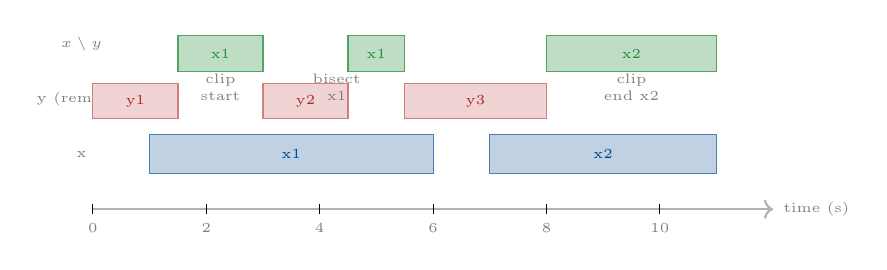
\begin{tikzpicture}[xscale=0.72]
  \draw[taxis] (0,-0.2)--(12,-0.2) node[right,font=\tiny,gray]{time (s)};
  \foreach \x in {0,2,...,10} \draw (\x,-0.14)--(\x,-0.26) node[tlabel,below]{\x};
  % x bars
  \node[font=\tiny,gray] at (-0.2,0.5) {x};
  \fill[bmlblue!25] (1,0.25) rectangle (6,0.75);   \draw[bmlblue!70] (1,0.25) rectangle (6,0.75);
  \node[font=\tiny,bmlblue] at (3.5,0.5) {x1};
  \fill[bmlblue!25] (7,0.25) rectangle (11,0.75);  \draw[bmlblue!70] (7,0.25) rectangle (11,0.75);
  \node[font=\tiny,bmlblue] at (9,0.5) {x2};
  % y bars
  \node[font=\tiny,gray] at (-0.2,1.2) {y (remove)};
  \fill[annotB!20] (0,0.95) rectangle (1.5,1.4);   \draw[annotB!60] (0,0.95) rectangle (1.5,1.4);
  \node[font=\tiny,annotB] at (0.75,1.17) {y1};
  \fill[annotB!20] (3,0.95) rectangle (4.5,1.4);   \draw[annotB!60] (3,0.95) rectangle (4.5,1.4);
  \node[font=\tiny,annotB] at (3.75,1.17) {y2};
  \fill[annotB!20] (5.5,0.95) rectangle (8,1.4);   \draw[annotB!60] (5.5,0.95) rectangle (8,1.4);
  \node[font=\tiny,annotB] at (6.75,1.17) {y3};
  % Result
  \node[font=\tiny,gray] at (-0.2,1.9) {$x \setminus y$};
  \fill[annotC!30] (1.5,1.55) rectangle (3,2.0);   \draw[annotC!80] (1.5,1.55) rectangle (3,2.0);
  \node[font=\tiny,annotC] at (2.25,1.775) {x1};
  \fill[annotC!30] (4.5,1.55) rectangle (5.5,2.0); \draw[annotC!80] (4.5,1.55) rectangle (5.5,2.0);
  \node[font=\tiny,annotC] at (5.0,1.775) {x1};
  \fill[annotC!30] (8,1.55) rectangle (11,2.0);    \draw[annotC!80] (8,1.55) rectangle (11,2.0);
  \node[font=\tiny,annotC] at (9.5,1.775) {x2};

  % Case labels
  \node[font=\tiny,gray,align=center] at (2.25,1.35) {clip\\start};
  \node[font=\tiny,gray,align=center] at (4.3,1.35) {bisect\\x1};
  \node[font=\tiny,gray,align=center] at (9.5,1.35) {clip\\end x2};
\end{tikzpicture}
\end{center}

Five geometric cases handled internally:
\begin{enumerate}[noitemsep]
  \item $y$ fully covers $x$ → $x$ row removed entirely
  \item $y$ clips the start of $x$ → fragment $[y.\text{ends},\; x.\text{ends}]$
  \item $y$ clips the end of $x$ → fragment $[x.\text{starts},\; y.\text{starts}]$
  \item $y$ bisects $x$ → two fragments: $[x.\text{starts},\;y.\text{starts}]$ and $[y.\text{ends},\;x.\text{ends}]$
  \item $y$ is outside $x$ → $x$ row kept as-is
\end{enumerate}

\begin{lstlisting}[style=matlab]
% Remove artifact periods from trial windows
clean_trials = bml_annot_difference(trial_windows, artifacts);
% Trials are split where artifacts bisect them.
% clean_trials.x_id_ links each fragment back to its original trial.

% Per-channel artifact removal (artifacts labelled by channel)
cfg = []; cfg.groupby_x = 'channel'; cfg.groupby_y = 'channel';
clean_per_ch = bml_annot_difference(cfg, lfp_windows, chan_artifacts);

% What remains after removing all high-gamma bursts from the session?
session_gaps = bml_annot_difference(session_window, hg_bursts);
\end{lstlisting}

% ============================================================
\section{bml\_annot\_consolidate --- Merging by Criterion}
\label{sec:consolidate}
% ============================================================

\subsection{Rationale}

Given a sorted annotation table, consolidate (merge) consecutive rows that satisfy a custom criterion. This is the most flexible grouping primitive in BML: it handles overlap merging, same-label grouping, fixed-size batching, and custom condition merging.

\subsection{Algorithm}

Starting from row 1, greedily try to add each next row to the current group $S$:
\begin{enumerate}[noitemsep]
  \item Tentatively add row $r$ to $S$
  \item Evaluate \texttt{criterion(S)}
  \item If true: keep $r$ in $S$, continue to next row
  \item If false: close current group, start new group with $r$
\end{enumerate}

The default criterion is overlap/contiguity: \texttt{criterion(S) = S.starts(end) <= max(S.ends(1:end-1))}.

\begin{center}
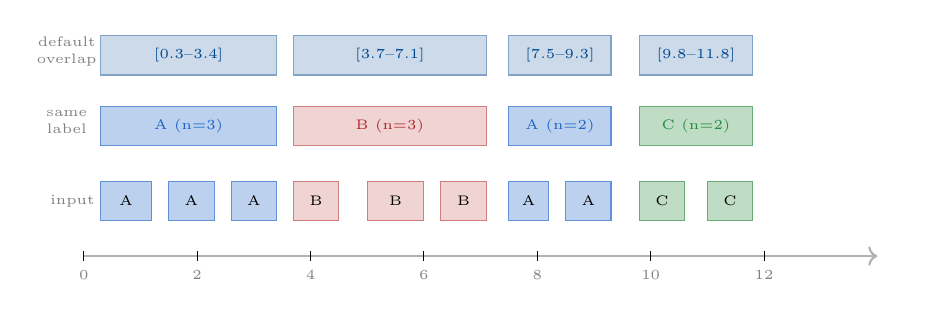
\begin{tikzpicture}[xscale=0.72]
  \draw[taxis] (0,-0.2)--(14,-0.2) node[right,font=\tiny,gray]{};
  \foreach \x in {0,2,...,12} \draw (\x,-0.14)--(\x,-0.26) node[tlabel,below]{\x};

  % Input: small bars with labels
  \node[font=\tiny,gray] at (-0.2,0.5) {input};
  \def\bars{{0.3/1.2/A},{1.5/2.3/A},{2.6/3.4/A},{3.7/4.5/B},{5.0/6.0/B},{6.3/7.1/B},
             {7.5/8.2/A},{8.5/9.3/A},{9.8/10.6/C},{11.0/11.8/C}}
  \foreach \s/\e/\lbl [count=\k] in {0.3/1.2/A, 1.5/2.3/A, 2.6/3.4/A, 3.7/4.5/B,
      5.0/6.0/B, 6.3/7.1/B, 7.5/8.2/A, 8.5/9.3/A, 9.8/10.6/C, 11.0/11.8/C}{
    \ifnum\k=1 \def\clr{annotA!30}\def\bclr{annotA!70}\fi
    \ifnum\k=2 \def\clr{annotA!30}\def\bclr{annotA!70}\fi
    \ifnum\k=3 \def\clr{annotA!30}\def\bclr{annotA!70}\fi
    \ifnum\k=4 \def\clr{annotB!20}\def\bclr{annotB!60}\fi
    \ifnum\k=5 \def\clr{annotB!20}\def\bclr{annotB!60}\fi
    \ifnum\k=6 \def\clr{annotB!20}\def\bclr{annotB!60}\fi
    \ifnum\k=7 \def\clr{annotA!30}\def\bclr{annotA!70}\fi
    \ifnum\k=8 \def\clr{annotA!30}\def\bclr{annotA!70}\fi
    \ifnum\k=9 \def\clr{annotC!30}\def\bclr{annotC!70}\fi
    \ifnum\k=10 \def\clr{annotC!30}\def\bclr{annotC!70}\fi
    \fill[\clr] (\s,0.25) rectangle (\e,0.75);
    \draw[\bclr] (\s,0.25) rectangle (\e,0.75);
    \node[font=\tiny] at ({(\s+\e)/2},0.5) {\lbl};
  }

  % Consolidation by same-label criterion
  \node[font=\tiny,gray,align=center] at (-0.3,1.5) {same\\label};
  % Group A (rows 1-3)
  \fill[annotA!30] (0.3,1.2) rectangle (3.4,1.7); \draw[annotA!70] (0.3,1.2) rectangle (3.4,1.7);
  \node[font=\tiny,annotA] at (1.85,1.45) {A (n=3)};
  % Group B (rows 4-6)
  \fill[annotB!20] (3.7,1.2) rectangle (7.1,1.7); \draw[annotB!60] (3.7,1.2) rectangle (7.1,1.7);
  \node[font=\tiny,annotB] at (5.4,1.45) {B (n=3)};
  % Group A again (rows 7-8)
  \fill[annotA!30] (7.5,1.2) rectangle (9.3,1.7); \draw[annotA!70] (7.5,1.2) rectangle (9.3,1.7);
  \node[font=\tiny,annotA] at (8.4,1.45) {A (n=2)};
  % Group C (rows 9-10)
  \fill[annotC!30] (9.8,1.2) rectangle (11.8,1.7);\draw[annotC!70] (9.8,1.2) rectangle (11.8,1.7);
  \node[font=\tiny,annotC] at (10.8,1.45) {C (n=2)};

  % Consolidation by default overlap
  \node[font=\tiny,gray,align=center] at (-0.3,2.4) {default\\overlap};
  \fill[bmlblue!20] (0.3,2.1) rectangle (3.4,2.6);  \draw[bmlblue!50] (0.3,2.1) rectangle (3.4,2.6);
  \node[font=\tiny,bmlblue] at (1.85,2.35) {[0.3--3.4]};
  \fill[bmlblue!20] (3.7,2.1) rectangle (7.1,2.6);  \draw[bmlblue!50] (3.7,2.1) rectangle (7.1,2.6);
  \node[font=\tiny,bmlblue] at (5.4,2.35) {[3.7--7.1]};
  \fill[bmlblue!20] (7.5,2.1) rectangle (9.3,2.6);  \draw[bmlblue!50] (7.5,2.1) rectangle (9.3,2.6);
  \node[font=\tiny,bmlblue] at (8.4,2.35) {[7.5--9.3]};
  \fill[bmlblue!20] (9.8,2.1) rectangle (11.8,2.6); \draw[bmlblue!50] (9.8,2.1) rectangle (11.8,2.6);
  \node[font=\tiny,bmlblue] at (10.8,2.35) {[9.8--11.8]};
\end{tikzpicture}
\end{center}

\begin{lstlisting}[style=matlab]
% 1. Default criterion: merge overlapping/touching (same as bml_annot_union)
cons = bml_annot_consolidate(annot);

% 2. Same-label grouping (like run-length encoding)
cfg = []; cfg.criterion = @(x) length(unique(x.label)) == 1;
cons_by_label = bml_annot_consolidate(cfg, annot);

% 3. Fixed group size (batch trials in groups of 4)
cfg = []; cfg.criterion = @(x) height(x) <= 4;
batches = bml_annot_consolidate(cfg, trials);

% 4. Contiguous files with same depth (NeuroOmega sync pattern)
cfg = [];
cfg.criterion = @(x) (length(unique(x.depth))==1) && ...
                     (abs((max(x.ends)-min(x.starts)) - sum(x.duration)) < 1e-2);
cons_depth = bml_annot_consolidate(cfg, neuro_info);

% Output columns always include:
%   cons_duration = sum(duration of merged rows)
%   id_starts     = id of first row in group
%   id_ends       = id of last row in group
%   cons_n        = number of rows merged
\end{lstlisting}

% ============================================================
\section{bml\_annot\_blocks --- Run-Length Encoding and Transitions}
\label{sec:blocks}
% ============================================================

\subsection{Rationale}

Given a sequence of annotations where each row has a label (e.g., a stimulus category, a behavioral state, a coding label), \texttt{bml\_annot\_blocks} groups consecutive rows with the \emph{same label} into blocks and records the \emph{transitions} between blocks. This is run-length encoding applied to time-series annotations.

\begin{center}
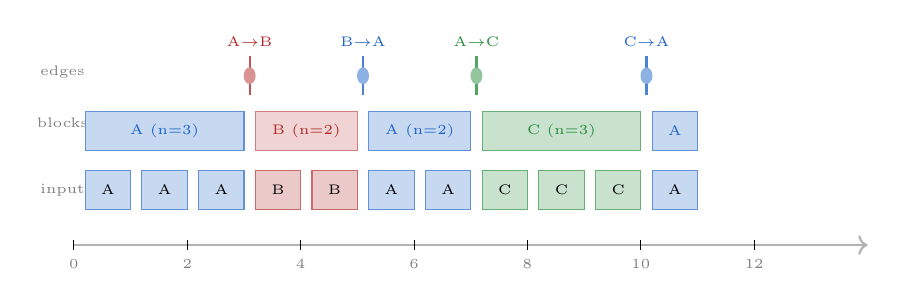
\begin{tikzpicture}[xscale=0.72]
  \draw[taxis] (0,-0.2)--(14,-0.2);
  \foreach \x in {0,2,...,12} \draw (\x,-0.14)--(\x,-0.26) node[tlabel,below]{\x};

  % Input label stream
  \node[font=\tiny,gray] at (-0.2,0.5) {input};
  \foreach \s/\e/\lbl/\clr in {
      0.2/1.0/A/annotA, 1.2/2.0/A/annotA, 2.2/3.0/A/annotA,
      3.2/4.0/B/annotB, 4.2/5.0/B/annotB,
      5.2/6.0/A/annotA, 6.2/7.0/A/annotA,
      7.2/8.0/C/annotC, 8.2/9.0/C/annotC, 9.2/10.0/C/annotC,
      10.2/11.0/A/annotA}{
    \fill[\clr!25] (\s,0.25) rectangle (\e,0.75);
    \draw[\clr!70] (\s,0.25) rectangle (\e,0.75);
    \node[font=\tiny] at ({(\s+\e)/2},0.5) {\lbl};
  }

  % Blocks output
  \node[font=\tiny,gray] at (-0.2,1.35) {blocks};
  \fill[annotA!25] (0.2,1.0) rectangle (3.0,1.5); \draw[annotA!70] (0.2,1.0) rectangle (3.0,1.5);
  \node[font=\tiny,annotA] at (1.6,1.25) {A (n=3)};
  \fill[annotB!20] (3.2,1.0) rectangle (5.0,1.5); \draw[annotB!60] (3.2,1.0) rectangle (5.0,1.5);
  \node[font=\tiny,annotB] at (4.1,1.25) {B (n=2)};
  \fill[annotA!25] (5.2,1.0) rectangle (7.0,1.5); \draw[annotA!70] (5.2,1.0) rectangle (7.0,1.5);
  \node[font=\tiny,annotA] at (6.1,1.25) {A (n=2)};
  \fill[annotC!25] (7.2,1.0) rectangle (10.0,1.5);\draw[annotC!70] (7.2,1.0) rectangle (10.0,1.5);
  \node[font=\tiny,annotC] at (8.6,1.25) {C (n=3)};
  \fill[annotA!25] (10.2,1.0) rectangle (11.0,1.5);\draw[annotA!70] (10.2,1.0) rectangle (11.0,1.5);
  \node[font=\tiny,annotA] at (10.6,1.25) {A};

  % Edges (transitions)
  \node[font=\tiny,gray] at (-0.2,2.0) {edges};
  \foreach \t/\pre/\post/\clr in {
      3.1/A/B/annotB, 5.1/B/A/annotA, 7.1/A/C/annotC, 10.1/C/A/annotA}{
    \draw[thick,\clr!80] (\t,1.7)--(\t,2.2);
    \fill[\clr!50] (\t,1.95) circle (3pt);
    \node[above,font=\tiny,\clr,align=center] at (\t,2.2) {\pre$\to$\post};
  }
\end{tikzpicture}
\end{center}

\begin{lstlisting}[style=matlab]
% Detect blocks of same stimulus condition
cfg = []; cfg.label = 'trial_type';
[blocks, edges] = bml_annot_blocks(cfg, trial_annot);
% blocks: id, starts, ends, duration, label, cons_n (how many rows merged)
% edges:  id, starts, ends, pre_label, post_label

% With win_edges: create a window around each transition
cfg = []; cfg.label = 'depth'; cfg.win_edges = 2.0; % ±2s window
[blocks, edges] = bml_annot_blocks(cfg, recording_info);
% edges.starts = transition_time - 2.0
% edges.ends   = transition_time + 2.0

% Group by an additional variable (e.g. per session)
cfg = []; cfg.label = 'state'; cfg.group_by = 'session_id';
[blocks, edges] = bml_annot_blocks(cfg, behavioral_coding);
\end{lstlisting}

% ============================================================
\section{bml\_annot\_shadow --- Filling the Gaps}
\label{sec:shadow}
% ============================================================

\subsection{Rationale}

Given a set of events, generate annotations that occupy the \emph{space between} them. The primary use case is creating pre-stimulus baselines: for each stimulus, get the silence that precedes it.

\begin{center}
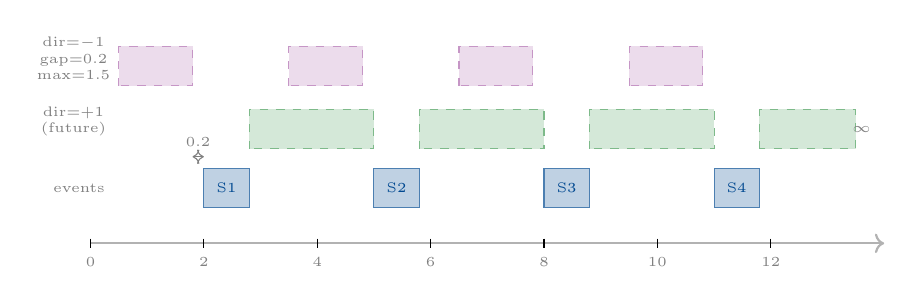
\begin{tikzpicture}[xscale=0.72]
  \draw[taxis] (0,-0.2)--(14,-0.2);
  \foreach \x in {0,2,...,12} \draw (\x,-0.14)--(\x,-0.26) node[tlabel,below]{\x};

  % Original events
  \node[font=\tiny,gray] at (-0.2,0.5) {events};
  \foreach \s/\e in {2/2.8, 5/5.8, 8/8.8, 11/11.8}{
    \fill[bmlblue!25] (\s,0.25) rectangle (\e,0.75);
    \draw[bmlblue!70] (\s,0.25) rectangle (\e,0.75);
  }
  \node[font=\tiny,bmlblue] at (2.4,0.5) {S1};
  \node[font=\tiny,bmlblue] at (5.4,0.5) {S2};
  \node[font=\tiny,bmlblue] at (8.4,0.5) {S3};
  \node[font=\tiny,bmlblue] at (11.4,0.5) {S4};

  % Forward shadow (gap=0, no max)
  \node[font=\tiny,gray,align=center] at (-0.3,1.35) {dir=+1\\(future)};
  \foreach \s/\e in {2.8/5, 5.8/8, 8.8/11}{
    \fill[annotC!20] (\s,1.0) rectangle (\e,1.5);
    \draw[annotC!60,dashed] (\s,1.0) rectangle (\e,1.5);
  }
  \fill[annotC!20] (11.8,1.0) rectangle (13.5,1.5);
  \draw[annotC!60,dashed] (11.8,1.0) rectangle (13.5,1.5);
  \node[font=\tiny,gray] at (13.6,1.25) {$\infty$};

  % Backward shadow (gap=0.2, max=1.5)
  \node[font=\tiny,gray,align=center] at (-0.3,2.15) {dir=$-1$\\gap=0.2\\max=1.5};
  \foreach \s/\e in {0.5/1.8, 3.5/4.8, 6.5/7.8, 9.5/10.8}{
    \fill[annotD!20] (\s,1.8) rectangle (\e,2.3);
    \draw[annotD!60,dashed] (\s,1.8) rectangle (\e,2.3);
  }
  % gap arrows
  \draw[<->,thin,gray] (1.8,0.9)--(2,0.9);
  \node[above,font=\tiny,gray] at (1.9,0.9) {0.2};
\end{tikzpicture}
\end{center}

\begin{lstlisting}[style=matlab]
% Pre-stimulus baseline: window before each stimulus (gap 0, max 1.5s)
cfg = [];
cfg.direction    = -1;      % look into the past
cfg.gap_duration = 0;       % shadow touches the event
cfg.max_duration = 1.5;     % cap at 1.5 s
baseline = bml_annot_shadow(cfg, stim_events);
% baseline(i).ends == stim_events(i).starts (gap=0)
% baseline(i).starts == stim_events(i).starts - min(1.5, gap_to_prev_event)

% Post-response silence (future direction, with 200 ms gap)
cfg = []; cfg.direction = 1; cfg.gap_duration = 0.2; cfg.max_duration = 2.0;
post_resp = bml_annot_shadow(cfg, response_events);

% The last shadow always extends to ±inf (clipped by max_duration if set).
% Use bml_annot_filter afterward to restrict to a session window:
post_resp = bml_annot_filter(post_resp, session_window);
\end{lstlisting}

% ============================================================
\section{bml\_annot\_coverage --- Measuring How Much is Covered}
\label{sec:coverage}
% ============================================================

\begin{formulabox}{Coverage formula}
$\mathrm{coverage}(y_j) = \dfrac{\displaystyle\sum_{i}\,|x_i \cap y_j|}{|y_j|}$

Returns a value in $[0,1]$: fraction of $y_j$'s duration covered by $x$.
\end{formulabox}

\begin{center}
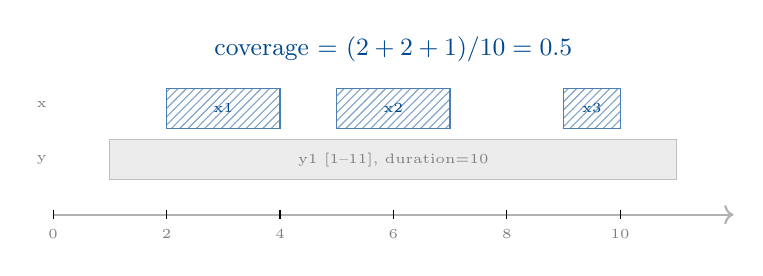
\begin{tikzpicture}[xscale=0.72]
  \draw[taxis] (0,-0.2)--(12,-0.2);
  \foreach \x in {0,2,...,10} \draw (\x,-0.14)--(\x,-0.26) node[tlabel,below]{\x};

  % y denominator bar
  \node[font=\tiny,gray] at (-0.2,0.5) {y};
  \fill[gray!15] (1,0.25) rectangle (11,0.75); \draw[gray!50] (1,0.25) rectangle (11,0.75);
  \node[font=\tiny,gray] at (6,0.5) {y1 [1--11], duration=10};

  % x numerator bars with hatching
  \node[font=\tiny,gray] at (-0.2,1.2) {x};
  \fill[bmlblue!30,pattern=north east lines,pattern color=bmlblue!50]
       (2,0.9) rectangle (4,1.4);
  \draw[bmlblue!70] (2,0.9) rectangle (4,1.4);
  \node[font=\tiny,bmlblue] at (3,1.15) {x1};
  \fill[bmlblue!30,pattern=north east lines,pattern color=bmlblue!50]
       (5,0.9) rectangle (7,1.4);
  \draw[bmlblue!70] (5,0.9) rectangle (7,1.4);
  \node[font=\tiny,bmlblue] at (6,1.15) {x2};
  \fill[bmlblue!30,pattern=north east lines,pattern color=bmlblue!50]
       (9,0.9) rectangle (10,1.4);
  \draw[bmlblue!70] (9,0.9) rectangle (10,1.4);
  \node[font=\tiny,bmlblue] at (9.5,1.15) {x3};

  % Coverage annotation
  \node[font=\small,bmlblue] at (6,1.9)
    {coverage = $(2+2+1)/10 = 0.5$};
\end{tikzpicture}
\end{center}

\begin{lstlisting}[style=matlab]
% Fraction of each trial covered by artifacts
cov = bml_annot_coverage(artifacts, trials);
% cov has same columns as trials plus 'coverage' (0 to 1)

% Keep only trials with < 10% artifact coverage
clean_trials = trials(cov.coverage < 0.1, :);

% Per-channel: artifact coverage per trial per channel
cfg = []; cfg.groupby_x = 'channel';
cov_per_ch = bml_annot_coverage(cfg, chan_artifacts, trials);
% One row per (trial x channel) combination

% Use custom column name
cfg = []; cfg.colname = 'artifact_fraction';
cov = bml_annot_coverage(cfg, artifacts, trials);
\end{lstlisting}

% ============================================================
\section{bml\_annot\_overlap --- Detecting Conflicts}
\label{sec:overlap}
% ============================================================

\texttt{bml\_annot\_overlap} finds all pairs of rows within the \emph{same} table that overlap each other. The result lists the overlapping pair IDs and the overlap region. Used for validation and debugging.

\begin{center}
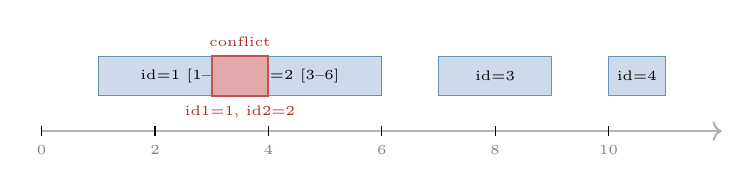
\begin{tikzpicture}[xscale=0.72]
  \draw[taxis] (0,-0.2)--(12,-0.2);
  \foreach \x in {0,2,...,10} \draw (\x,-0.14)--(\x,-0.26) node[tlabel,below]{\x};

  % 4 annotation bars, 2 overlapping
  \fill[bmlblue!20] (1,0.25) rectangle (4,0.75);  \draw[bmlblue!60] (1,0.25) rectangle (4,0.75);
  \node[font=\tiny] at (2.5,0.5) {id=1 [1--4]};
  \fill[bmlblue!20] (3,0.25) rectangle (6,0.75);  \draw[bmlblue!60] (3,0.25) rectangle (6,0.75);
  \node[font=\tiny] at (4.5,0.5) {id=2 [3--6]};
  \fill[bmlblue!20] (7,0.25) rectangle (9,0.75);  \draw[bmlblue!60] (7,0.25) rectangle (9,0.75);
  \node[font=\tiny] at (8,0.5) {id=3};
  \fill[bmlblue!20] (10,0.25) rectangle (11,0.75);\draw[bmlblue!60] (10,0.25) rectangle (11,0.75);
  \node[font=\tiny] at (10.5,0.5) {id=4};

  % Conflict region
  \fill[annotB!40] (3,0.25) rectangle (4,0.75);
  \draw[annotB!80,thick] (3,0.25) rectangle (4,0.75);
  \node[above,font=\tiny,annotB] at (3.5,0.75) {conflict};
  \node[below,font=\tiny,annotB] at (3.5,0.25) {id1=1, id2=2};
\end{tikzpicture}
\end{center}

\begin{lstlisting}[style=matlab]
% Validate that a table has no overlaps (required before passing as y to intersect)
ovlp = bml_annot_overlap(annot);
assert(isempty(ovlp), 'Table has %d overlapping pairs', height(ovlp));

% Find and inspect overlapping pairs
ovlp = bml_annot_overlap(my_events);
if ~isempty(ovlp)
  disp(ovlp);  % id1, id2, starts, ends of each overlap
  % Fix: resolve by merging or trimming conflicting rows
  my_events = bml_annot_union(my_events);  % merge overlapping pairs
end
\end{lstlisting}

% ============================================================
\section{Joining Tables}
\label{sec:joins}
% ============================================================

\subsection{bml\_annot\_left\_join --- Key-Based Join}

Standard relational left join: all rows of the left table are preserved; columns from the right table are added where the key matches.

\begin{lstlisting}[style=matlab]
% Add subject/session metadata to each trial
cfg = []; cfg.keys = {'session_id'};
trials_with_meta = bml_annot_left_join(cfg, trials, session_metadata);

% Add per-electrode impedance to spike annotations
cfg = []; cfg.keys = {'channel'};
spikes_full = bml_annot_left_join(cfg, spikes, electrode_info);
\end{lstlisting}

\subsection{bml\_annot\_transfer --- Temporal Overlap Join}

For each row in \texttt{annot}, find which row(s) in \texttt{transfer} contain it (by time overlap), and copy selected columns. Useful for assigning epoch-level labels to individual events within the epoch.

\begin{center}
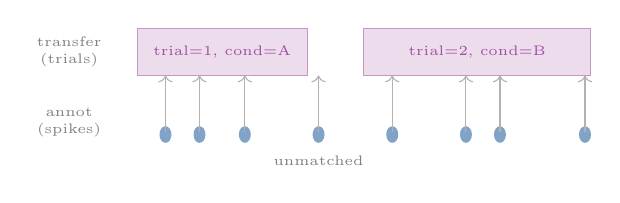
\begin{tikzpicture}[xscale=0.72]
  % Events (annot)
  \node[font=\tiny,gray,align=center] at (-0.2,0.5) {annot\\(spikes)};
  \foreach \t in {1.5,2.1,2.9,4.2,5.5,6.8,7.4,8.9}{
    \fill[bmlblue!50] (\t,0.35) circle (3pt);
  }
  % Transfer table (epochs)
  \node[font=\tiny,gray,align=center] at (-0.2,1.4) {transfer\\(trials)};
  \fill[annotD!20] (1,1.1) rectangle (4,1.7);  \draw[annotD!60] (1,1.1) rectangle (4,1.7);
  \node[font=\tiny,annotD] at (2.5,1.4) {trial=1, cond=A};
  \fill[annotD!20] (5,1.1) rectangle (9,1.7);  \draw[annotD!60] (5,1.1) rectangle (9,1.7);
  \node[font=\tiny,annotD] at (7.0,1.4) {trial=2, cond=B};
  % Arrows
  \foreach \t/\tr in {1.5/1, 2.1/1, 2.9/1, 4.2/?, 5.5/2, 6.8/2, 7.4/2, 8.9/2}{
    \draw[->,thin,gray!60] (\t,0.38)--(\t,1.1);
  }
  \node[below,font=\tiny,gray] at (4.2,0.2) {unmatched};
\end{tikzpicture}
\end{center}

\begin{lstlisting}[style=matlab]
% Assign trial condition label to each spike
cfg = []; cfg.select = {'trial_id','condition','response'};
spikes_labeled = bml_annot_transfer(cfg, spikes, trial_epochs);
% Each spike gets the trial_id/condition/response of the trial containing it.
% Spikes not inside any trial get NaN/empty for transferred columns.

% cfg.overlap: require spike to be at least 50% inside the epoch
cfg.overlap = 0.5;
\end{lstlisting}

% ============================================================
\section{bml\_annot\_calculate --- Feature Extraction over Epochs}
\label{sec:calculate}
% ============================================================

Applies scalar functions to raw signal data over each epoch defined by an annotation table. Each function receives a \texttt{FT\_DATATYPE\_RAW} segment and must return a scalar (or one scalar per channel).

\begin{lstlisting}[style=matlab]
% Define feature functions
rms_fn   = @(raw) sqrt(mean(raw.trial{1}(1,:).^2));
peak2pk  = @(raw) max(raw.trial{1}(1,:)) - min(raw.trial{1}(1,:));
log_pwr  = @(raw) 10*log10(mean(raw.trial{1}(1,:).^2));

% Compute features for each trial
cfg = [];
cfg.roi   = sync_roi(strcmp(sync_roi.filetype,'trellis'),:);
cfg.epoch = trial_windows;
trial_features = bml_annot_calculate(cfg, trial_windows, ...
  'rms', rms_fn, 'peak2peak', peak2pk, 'log_power', log_pwr);
% trial_features has all original columns plus rms, peak2peak, log_power

% bml_annot_describe: summary statistics per group
cfg = []; cfg.groupby = 'condition';
stats = bml_annot_describe(cfg, trial_features);
% stats: condition, variable, mean, median, std, min, max, count
\end{lstlisting}

% ============================================================
\section{bml\_annot\_detect --- Threshold-Based Event Detection}
\label{sec:detect}
% ============================================================

Detects epochs where a signal exceeds a threshold. The algorithm finds peaks above the upper threshold, then expands each detection to the nearest zero-crossing of the lower threshold.

\begin{center}
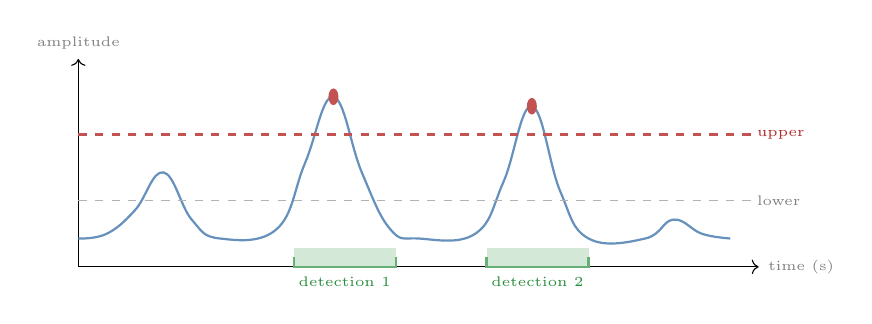
\begin{tikzpicture}[xscale=0.72, yscale=1.2]
  \draw[->] (0,-0.2)--(12,-0.2) node[right,font=\tiny,gray]{time (s)};
  \draw[->] (0,-0.2)--(0,2.0) node[above,font=\tiny,gray]{amplitude};
  % Signal (approximate sine-like bumps)
  \draw[bmlblue!60, thick] plot[smooth,tension=0.7] coordinates{
    (0,0.1)(0.5,0.15)(1,0.4)(1.5,0.8)(2,0.3)(2.5,0.1)
    (3.5,0.2)(4,0.9)(4.5,1.6)(5,0.8)(5.5,0.2)
    (6,0.1)(7,0.15)(7.5,0.7)(8,1.5)(8.5,0.6)(9,0.1)
    (10,0.1)(10.5,0.3)(11,0.15)(11.5,0.1)
  };
  % Upper threshold
  \draw[annotB!80,dashed,thick] (0,1.2)--(12,1.2);
  \node[right,font=\tiny,annotB] at (11.8,1.2) {upper};
  % Lower threshold
  \draw[gray!60,dashed] (0,0.5)--(12,0.5);
  \node[right,font=\tiny,gray] at (11.8,0.5) {lower};
  % Detected events (shaded)
  \fill[annotC!20] (3.8,-0.2) rectangle (5.6,0);
  \draw[annotC!70,thick] (3.8,-0.1)--(3.8,-0.2)--(5.6,-0.2)--(5.6,-0.1);
  \node[below,font=\tiny,annotC] at (4.7,-0.2) {detection 1};
  \fill[annotC!20] (7.2,-0.2) rectangle (9.0,0);
  \draw[annotC!70,thick] (7.2,-0.1)--(7.2,-0.2)--(9.0,-0.2)--(9.0,-0.1);
  \node[below,font=\tiny,annotC] at (8.1,-0.2) {detection 2};
  % Peak marker
  \fill[annotB!80] (4.5,1.6) circle (2.5pt);
  \fill[annotB!80] (8,1.5) circle (2.5pt);
\end{tikzpicture}
\end{center}

\begin{lstlisting}[style=matlab]
% Detect high-gamma (HG) bursts above 3 std
hg_raw = bml_load_continuous(struct('roi', hg_roi));

cfg = [];
cfg.threshold   = [1.0, 3.0];  % [lower, upper] in units of the signal
cfg.channel     = 'G14';
cfg.max_annots  = 500;
hg_bursts = bml_annot_detect(cfg, hg_raw);
% hg_bursts: starts, ends, env_max, trial, label

% Single threshold (upper only; lower = 0 crossing)
cfg = []; cfg.threshold = 3.0;
detections = bml_annot_detect(cfg, envelope_raw);
\end{lstlisting}

% ============================================================
\section{bml\_annot2raw / bml\_raw2annot --- Signal Encoding}
\label{sec:encoding}
% ============================================================

\subsection{Annotations to binary/count signals (\texttt{bml\_annot2raw})}

Converts an annotation table to a continuous FT\_DATATYPE\_RAW signal: 1 where a row covers that sample, 0 elsewhere. With \texttt{cfg.count=true}, counts overlapping annotations per sample.

\begin{center}
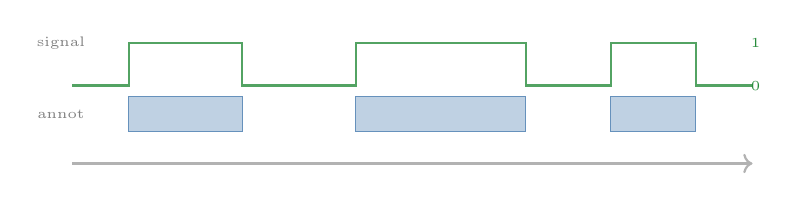
\begin{tikzpicture}[xscale=0.72, yscale=0.9]
  \draw[taxis] (0,-0.2)--(12,-0.2);
  % Annotation bars
  \node[font=\tiny,gray] at (-0.2,0.5) {annot};
  \fill[bmlblue!25] (1,0.25) rectangle (3,0.75); \draw[bmlblue!60] (1,0.25) rectangle (3,0.75);
  \fill[bmlblue!25] (5,0.25) rectangle (8,0.75); \draw[bmlblue!60] (5,0.25) rectangle (8,0.75);
  \fill[bmlblue!25] (9.5,0.25) rectangle (11,0.75); \draw[bmlblue!60] (9.5,0.25) rectangle (11,0.75);
  % Binary signal
  \node[font=\tiny,gray] at (-0.2,1.5) {signal};
  \draw[annotC!80,thick] (0,0.9)--(1,0.9)--(1,1.5)--(3,1.5)--(3,0.9)--
    (5,0.9)--(5,1.5)--(8,1.5)--(8,0.9)--
    (9.5,0.9)--(9.5,1.5)--(11,1.5)--(11,0.9)--(12,0.9);
  \node[right,font=\tiny,annotC] at (11.8,0.9) {0};
  \node[right,font=\tiny,annotC] at (11.8,1.5) {1};
\end{tikzpicture}
\end{center}

\begin{lstlisting}[style=matlab]
% Create binary stimulus presence signal (for cross-correlation with neural data)
cfg = [];
cfg.roi         = trellis_roi;
cfg.label       = 'stim_channel';
stim_raw = bml_annot2raw(cfg, stim_annotations);

% Count overlapping artifacts per sample (for quality metric)
cfg = []; cfg.count = true;
artifact_count_raw = bml_annot2raw(cfg, artifacts, trellis_roi);
% Each sample = number of simultaneously overlapping artifact annotations

% Per-label channels: one channel per unique label value
cfg = []; cfg.label_colname = 'trial_type';
coding_raw = bml_annot2raw(cfg, trial_annotations, roi);
% coding_raw has one channel per trial_type

% Inverse: extract time bounds from a raw struct back to annotation metadata
annot_meta = bml_raw2annot([], lfp_raw);
% annot_meta: starts, ends, trial, s1, t1, s2, t2, Fs, nSamples
\end{lstlisting}

% ============================================================
\section{bml\_annot\_plot --- Visualization}
\label{sec:plot}
% ============================================================

Plots annotation intervals as horizontal line segments, with optional faceting (subplots) and y-axis grouping.

\begin{lstlisting}[style=matlab]
% Basic: one line per annotation id
bml_annot_plot([], trial_windows);

% Group by trial_type on y-axis
cfg = []; cfg.y = 'trial_type';
bml_annot_plot(cfg, trial_windows);

% Facet by session (one subplot per session)
cfg = [];
cfg.y     = 'channel';    % y-axis = channel number
cfg.facet = 'session_id'; % one panel per session
bml_annot_plot(cfg, lfp_epochs);

% Use in a pipeline to inspect intermediate results
bml_annot_plot([], bml_annot_filter(events, session));
\end{lstlisting}

% ============================================================
\section{bml\_annot\_t0 and bml\_annot\_rowbind --- Utilities}
\label{sec:utils}
% ============================================================

\subsection{bml\_annot\_t0 --- Change Time Reference}

Shifts all times by a constant. Used when you need times relative to an event (e.g., stimulus onset = 0).

\begin{formulabox}{Time shift}
$\texttt{starts}_{\rm new} = \texttt{starts} - t_0,\quad
 \texttt{ends}_{\rm new} = \texttt{ends} - t_0$
\end{formulabox}

\begin{lstlisting}[style=matlab]
% Set stimulus onset as t=0
cfg = []; cfg.t0 = stim_events.starts(trial_idx);
relative_events = bml_annot_t0(cfg, all_events);

% Use roi.starts as reference (common in per-file analysis)
cfg = []; cfg.roi = roi(file_idx,:);
relative = bml_annot_t0(cfg, events_in_file);
\end{lstlisting}

\subsection{bml\_annot\_rowbind --- Vertical Concatenation}

Concatenates multiple annotation tables, conforming all to the schema of the first non-empty table (fills missing columns with appropriate empty values).

\begin{lstlisting}[style=matlab]
% Combine sync results from three methods
all_sync = bml_annot_rowbind(sync_roi_analog, sync_roi_no, sync_roi_ptb);

% Safer than [A; B; C] because it handles schema mismatches gracefully
% (missing columns are filled with NaN/empty)
\end{lstlisting}

% ============================================================
\section{Complete Worked Example: From Raw Events to Clean Trial Features}
\label{sec:example}
% ============================================================

This example walks through a complete analysis pipeline using all the major annotation operations. Goal: extract high-gamma power from clean trial windows, per condition.

\begin{center}
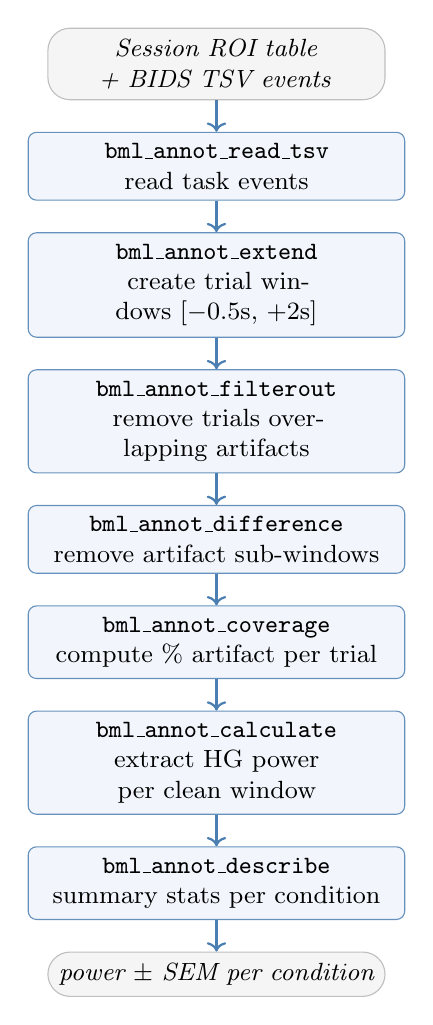
\begin{tikzpicture}[
  fn/.style={rectangle, rounded corners=3pt, draw=bmlblue!60, fill=boxbg,
             text width=4.5cm, align=center, inner sep=4pt, font=\small},
  data/.style={rectangle, rounded corners=8pt, draw=gray!50, fill=gray!8,
               text width=4.0cm, align=center, inner sep=4pt, font=\small\itshape},
  arr/.style={->, thick, bmlblue!70},
  node distance=0.4cm
]
  \node[data] (raw) {Session ROI table\\+ BIDS TSV events};
  \node[fn, below=of raw] (f1) {\texttt{bml\_annot\_read\_tsv}\\read task events};
  \node[fn, below=of f1] (f2) {\texttt{bml\_annot\_extend}\\create trial windows [$-$0.5s, +2s]};
  \node[fn, below=of f2] (f3) {\texttt{bml\_annot\_filterout}\\remove trials overlapping artifacts};
  \node[fn, below=of f3] (f4) {\texttt{bml\_annot\_difference}\\remove artifact sub-windows};
  \node[fn, below=of f4] (f5) {\texttt{bml\_annot\_coverage}\\compute \% artifact per trial};
  \node[fn, below=of f5] (f6) {\texttt{bml\_annot\_calculate}\\extract HG power per clean window};
  \node[fn, below=of f6] (f7) {\texttt{bml\_annot\_describe}\\summary stats per condition};
  \node[data, below=of f7] (out) {power $\pm$ SEM per condition};
  \foreach \a/\b in {raw/f1, f1/f2, f2/f3, f3/f4, f4/f5, f5/f6, f6/f7, f7/out}
    \draw[arr] (\a) -- (\b);
\end{tikzpicture}
\end{center}

\begin{lstlisting}[style=matlab, caption={Complete pipeline: raw events to trial features}]
%% STEP 1: Load session ROI and build sync
roi = bml_roi_table(bml_info_raw(struct('folder',PATH_DATA)));
sync_roi = load(fullfile(PATH_SYNC,'sync_roi_final.mat')); % pre-computed

%% STEP 2: Read task events (BIDS TSV)
events = bml_annot_read_tsv( ...
  'sub-DM1001_ses-intraop_task-speech_events.tsv');
% events.starts = master-clock time (after sync applied at recording)
% events.trial_type = {'go','nogo','go',...}

%% STEP 3: Create trial analysis windows
% Each trial = 0.5s before onset to 2s after
trial_windows = bml_annot_extend(events, 0.5, 2.0);
fprintf('Total trials: %d\n', height(trial_windows));

%% STEP 4: Load artifact annotations
artifacts = bml_annot_read_tsv('artifacts.tsv');
artifacts = bml_annot_filter(artifacts, session_window); % keep session-range only

%% STEP 5: Remove trials that are >50% artifact
cfg_filt = []; cfg_filt.overlap = 0.5;
clean_trials = bml_annot_filterout(cfg_filt, trial_windows, artifacts);
fprintf('Trials after artifact rejection: %d / %d\n', ...
  height(clean_trials), height(trial_windows));

%% STEP 6: Compute per-trial artifact coverage
cov = bml_annot_coverage(artifacts, clean_trials);
clean_trials.artifact_pct = cov.coverage * 100;

%% STEP 7: Get clean (non-artifact) sub-windows for each trial
clean_windows = bml_annot_difference(clean_trials, artifacts);
% clean_windows.x_id_ links back to original trial id

%% STEP 8: Transfer trial metadata to clean windows
cfg_tr = []; cfg_tr.select = {'trial_type','value','session_id'};
clean_windows = bml_annot_transfer(cfg_tr, clean_windows, clean_trials);

%% STEP 9: Compute high-gamma power in each clean window
hg_roi = sync_roi(strcmp(sync_roi.filetype,'trellis') & ...
                  strcmp(sync_roi.chantype,'hg'),:);

log_pwr = @(raw) 10*log10(mean(raw.trial{1}(1,:).^2) + eps);

cfg_calc = []; cfg_calc.roi = hg_roi;
results = bml_annot_calculate(cfg_calc, clean_windows, ...
  'log_power_hg', log_pwr);

%% STEP 10: Descriptive stats per condition
cfg_desc = []; cfg_desc.groupby = 'trial_type';
stats = bml_annot_describe(cfg_desc, results);
disp(stats);  % trial_type | variable | mean | std | count | ...

%% STEP 11: Visualize
cfg_plot = []; cfg_plot.y = 'trial_type'; cfg_plot.facet = 'session_id';
bml_annot_plot(cfg_plot, clean_trials);
title('Clean trials by condition');
\end{lstlisting}

% ============================================================
\section{Annotation Algebra: Complete Reference Table}
\label{sec:reference}
% ============================================================

\begin{center}
\small
\begin{longtable}{L{3.5cm} L{2.5cm} L{3.5cm} L{4cm}}
\toprule
\textbf{Function} & \textbf{Operation} & \textbf{What it does} & \textbf{Typical use} \\
\midrule
\endhead
\texttt{bml\_annot\_table} & Constructor & Enforce schema, sort by starts, recompute duration & Create any annotation table \\
\texttt{bml\_roi\_table} & Constructor & Extend with file metadata + (s1,t1,s2,t2) & Build file/session index \\
\texttt{bml\_annot\_read\_tsv} & I/O & Load BIDS TSV event files & Load task event logs \\
\texttt{bml\_annot\_write\_tsv} & I/O & Save as BIDS TSV & Export synced events \\
\texttt{bml\_event2annot} & Conversion & FieldTrip events $\to$ annotation table & Convert Ripple events \\
\texttt{bml\_annot2raw} & Encoding & Annotations $\to$ binary/count signal & Cross-correlation, QC \\
\texttt{bml\_raw2annot} & Encoding & Raw struct $\to$ time metadata & Extract file coordinates \\
\texttt{bml\_annot\_extend} & Dilation/Erosion & Expand or shrink interval boundaries & Analysis windows, coarsetol \\
\texttt{bml\_annot\_filter} & Selection & Keep rows that overlap a window & Restrict to session/ROI \\
\texttt{bml\_annot\_filterout} & Exclusion & Remove rows that overlap a window & Artifact rejection \\
\texttt{bml\_annot\_intersect} & Intersection & Clip to overlap region, track parent IDs & Find overlapping epochs \\
\texttt{bml\_annot\_union} & Union & Merge overlapping/touching intervals & Combine artifact lists \\
\texttt{bml\_annot\_difference} & Subtraction & Remove $y$ from $x$, split intervals & Clean trial windows \\
\texttt{bml\_annot\_consolidate} & Grouping & Merge by custom criterion function & Run-length, batch, overlap \\
\texttt{bml\_annot\_blocks} & RLE & Contiguous same-label runs + transitions & Behavioral state segmentation \\
\texttt{bml\_annot\_shadow} & Gap filling & Annotations in the gaps between events & Pre/post-stimulus baseline \\
\texttt{bml\_annot\_coverage} & Measurement & Fraction of $y$ covered by $x$ & Artifact quality metric \\
\texttt{bml\_annot\_overlap} & Validation & Find conflicting (overlapping) pairs & Schema validation \\
\texttt{bml\_annot\_left\_join} & Join & Key-based relational join & Add metadata columns \\
\texttt{bml\_annot\_transfer} & Temporal join & Copy columns based on time overlap & Assign trial labels to spikes \\
\texttt{bml\_annot\_calculate} & Aggregation & Apply functions to raw data per epoch & Feature extraction \\
\texttt{bml\_annot\_describe} & Statistics & Descriptive stats per group & Summarize features \\
\texttt{bml\_annot\_detect} & Detection & Threshold-crossing event detection & Detect HG bursts, peaks \\
\texttt{bml\_annot\_match} & Template match & Cross-correlation peak detection & Find pattern occurrences \\
\texttt{bml\_annot\_t0} & Translation & Shift all times by a constant & Event-relative time axis \\
\texttt{bml\_annot\_rowbind} & Concatenation & Vertical concat with schema conforming & Merge tables from loops \\
\texttt{bml\_annot\_conform\_to} & Schema & Align column schema to template & Pre-concatenation fix \\
\texttt{bml\_annot\_rename} & Projection & Rename columns & Column name cleanup \\
\texttt{bml\_annot\_sample} & Sampling & Random row selection & Subsampling for tests \\
\texttt{bml\_annot\_plot} & Visualization & Horizontal bar plot, faceted & Inspect epoch tables \\
\bottomrule
\end{longtable}
\end{center}

% ============================================================
\appendix
\section{Interval Algebra: Mathematical Summary}
% ============================================================

\subsection*{Notation}
$A = [a_1, a_2]$, $B = [b_1, b_2]$, $|A| = a_2 - a_1$.

\subsection*{Overlap condition}
$A \cap B \neq \emptyset \;\Leftrightarrow\; a_1 < b_2 \text{ and } a_2 > b_1$

\subsection*{Intersection}
$A \cap B = [\max(a_1,b_1),\; \min(a_2,b_2)]$, valid when non-empty.

\subsection*{Union (two intervals)}
$A \cup B = [\min(a_1,b_1),\; \max(a_2,b_2)]$ when they overlap or touch ($b_1 \leq a_2 + \varepsilon$).

\subsection*{Difference}
$A \setminus B$: the part of $A$ not covered by $B$. May produce 0, 1, or 2 intervals.

\subsection*{Extension/Erosion}
$\mathrm{extend}(A, e_1, e_2) = [a_1 - e_1,\; a_2 + e_2]$. Positive = dilate; negative = erode.

\subsection*{Coverage}
$\mathrm{cov}(X, y) = \dfrac{\sum_i |X_i \cap y|}{|y|}$, where $X = \{X_i\}$ is a set of intervals.

\subsection*{Index $\leftrightarrow$ time (ROI coordinates)}
$F_{s,\mathrm{eff}} = \tfrac{s_2-s_1}{t_2-t_1}$, \quad
$t(i) = \tfrac{i}{F_{s,\mathrm{eff}}} - \tfrac{0.5}{F_{s,\mathrm{eff}}} + \tfrac{s_2 t_1 - t_2 s_1}{s_2-s_1}$, \quad
$i(t) = \mathrm{round}\!\bigl(\tfrac{t_2 s_1 - s_2 t_1 + (s_2-s_1)\,t}{t_2-t_1}\bigr)$

\vfill
\begin{center}
{\small\color{gray}
Brain Modulation Laboratory $\cdot$ Massachusetts General Hospital $\cdot$ April 2026}
\end{center}
\end{document}

